%!TEX root = ../main.tex
% mainfile: ../main.tex

\section{Formalisms}

\subsection{Basics}
\begin{figure}[th]
\centering
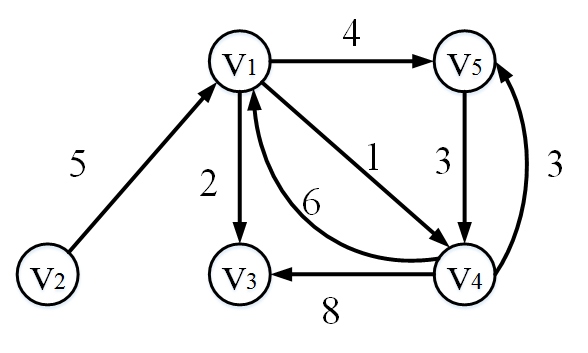
\includegraphics[width=2.4in]{figures/mention_network.png} %?????????????
\caption{An example mentions network. Nodes denote Twitter users,
directed edges denote direction of mentions between users, and edges
are labeled with mention frequency.}
\label{fig:mention_network}
\end{figure}

We model Twitter activity as a network $G(V,E)$ of mentions.
Here, each vertex $v \in V$ represents a Twitter user.
There is a directed edge from user $v_i$ to user $v_j$
if $v_i$ mentions $v_j$ in
a tweet.
We define $\omega_{ij}$ to be the number of tweets in which user $v_i$ mentions user $v_j$. Note that $\omega_{ij}$ is not necessarily equal to $\omega_{ji}$.
Key players such as celebrities and politicians are more
likely to be mentioned by other users, rather than the other way around.
As can be seen in Fig.~\ref{fig:mention_network}, the mentions network
is a directed graph. Weight $w_{14}$ is the number of times Twitter user $v_1$ mentions user $v_4$, which is 1, while $w_{41}$ is 6. Note
that $w_{21}$ is 5, while $w_{12}$ is 0 (not shown).

We define the neighborhood $N(v_i)$ of a user $v_i$ as the set of all users
mentioned by $v_i$, i.e., those for whom there is a directed edge from
$v_i$.
For each user $v_j \in N(v_i)$, we define the Brownian distance from user $v_i$ to $v_j$ to be
\begin{equation}
 d_{ij}=\frac{1}{(\omega_{ij}+1)(\omega_{ji}+1)^\gamma(\eta_{ij}+1)^\gamma}
\end{equation}
Here, $\eta_{ij}$ is the number of common direct neighbors shared by user $v_i$ and user $v_j$~\cite{zhou2004network}. In Fig.~\ref{fig:mention_network}, node $v_1$ and $v_4$ share two common direct neighbors---$v_3$ and $v_5$---and
hence $\eta_{14}$ is 2.

We use the bias coefficient $\gamma \geq 1$ to heuristically
weigh mentions that carry more impact. If $v_i$ mentions $v_j$, meaning that $\omega_{ij} > 0$, we believe this expresses $v_i$'s intention to propagate information to $v_j$.
Since $v_j$ may not know or care about $v_i$ and consequently may seldom or never mention $v_i$, the return mentions, measured by $\omega_{ji}$, are (up)weighted by $\gamma$.
Furthermore, if $v_i$ and $v_j$ share neighbors in the mentions
network, the two users may have a closer relationship than other users
with no shared mentioned Twitter users, and thus this component
is weighted by $\gamma$ as well. A Laplacian-style $(+1)$ correction is used
when there are no counter mentions or no mutual mentions.
Note that for $\gamma = 1$, $d_{ij}$ is an unbiased Brownian distance since $\omega_{ij}$, $\omega_{ji}$, and $\eta_{ij}$ will have the same weight.

\subsection{Trust functions and GBM}
\begin{figure}[ht]
\centering
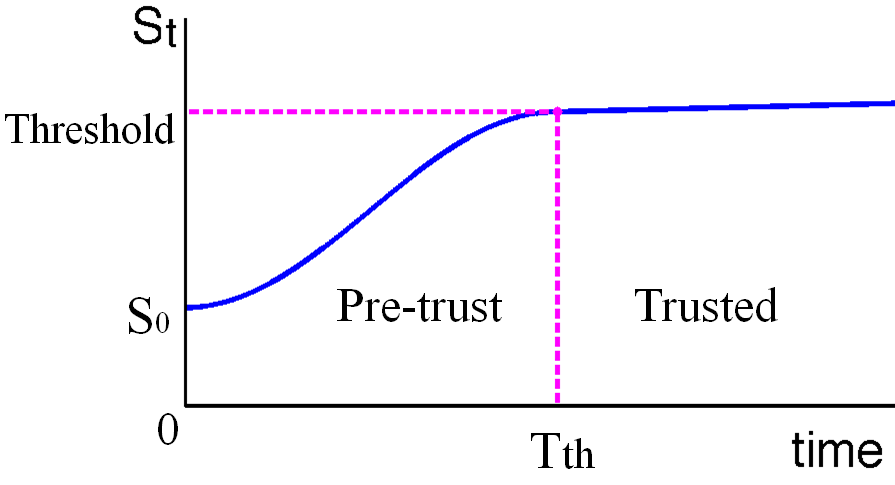
\includegraphics[width=2.4in, height=1.4in]{figures/trustFunction.png} %?????????????
\caption{Trust function. A threshold defines the transition between the
pre-trust and trusted period.}
\label{fig:subgraph}
\end{figure}

Next we introduce the notion of a
trust function $S_t$ which we use to model an individual user's agreement with an idea as expressed in tweets.
(The trust function $S_t$ is a function of the two entities between whom
trust is modeled, but in this section we simplify the notation for
ease of exposition.)
We divide the trust process into a pre-trust
period and a trusted period.
In the pre-trust period, as a user receives new information, that user's trust, $S_t$, increases exponentially until $S_t$ reaches the trust threshold at time $T_{th}$ and enters the trusted period.
In the trusted period, new information increases $S_t$ linearly. For simplicity, an individual user cannot revoke trust once this threshold has been crossed. In our Twitter mentions network, a user's trust in a topic crosses the threshold when they have tweeted about it. During the pre-trust period, we model the
trust function as follows (the coefficient $\mu$ accounts for change in the average value of this stochastic process):
\begin{equation}\frac{d S_t}{S_t} = \mu {dt}\end{equation}
% introduce $\sigma$, $W_t$


We then add a Wiener process $W_t$ to account for stochasticity.
According to the properties of a Wiener process~\cite{oksendal2003stochastic},
$dW_t$ is essentially Gaussian white noise and contributes to our
equation as:
\begin{equation}\frac{d S_t}{S_t} = \mu {dt}+\sigma dW_t\end{equation}
In this way, we modeled the trust function $S_t$ as a geometric Brownian motion (GBM) process which is a continuous-time stochastic process~\cite{oksendal2003stochastic}. Per convention, we call $\mu$ the drift and $\sigma$ the volatility. The drift represents deterministic trends while the volatility refers to the influence of unpredictable events in this model~\cite{wiersema2008brownian}. For simplicity, we consider $\mu$ and $\sigma$ to be constant during the pre-trust period in this chapter. (Our concern here primarily is with this period.)


According to It\={o}'s theorem~\cite{oksendal2003stochastic}, given the initial value $S_0$,
the above stochastic differential equation has the following analytic solution:
\begin{equation}
S_{t}=S_{0}\exp \left(\left(\mu -{\frac  {\sigma ^{2}}{2}}\right)t+\sigma W_{t}\right)
\end{equation}
The above solution for $S_{t}$ is a log-normally distributed random variable with expected value and variance given as~\cite{oksendal2003stochastic}:
\begin{equation}
{  {E}}(S_{t})=S_0e^{{\mu t}}
\end{equation}
\vspace{-1em}
\begin{equation}
 {Var}(S_{t})=S_0^2e^{{2\mu t}}\left(e^{{\sigma ^{2}t}}-1\right)
\end{equation} $S_t$ is a geometric Brownian motion stochastic process, which is typically denoted as $\mathcal{B}(\mu,\sigma)$.
In this chapter we use an initial trust of $S_0 = 1$ without loss of generality.



%\begin{algorithm}
%\label{alg:gbm_prop}
%\SetKwData{Left}{left}\SetKwData{This}{this}\SetKwData{Up}{up}
%\SetKwFunction{Union}{Union}\SetKwFunction{FindCompress}{FindCompress}
%\SetKwInOut{Input}{input}\SetKwInOut{Output}{output}
%\SetAlgoLined
%\Input{mentions network $G(V,E)$, time step $\delta t$, propagation time $T$}
%\Output{infected users}
%        \For{\textrm{each infected user} $v_i \in V$}
%	{	
%	 \For{\textrm{each non-infected user} $v_j \in N(v_i)$}
%	   { set $t_{ij}=0$;}
%	     set $v_i$ as \textrm{not newly infected user}
%        }
% t = 0; \\
%\For{$t \leq T$}{
%    \For{each infected user $v_i \in V$}
%	{  \If{$v_i$ is \textrm{a newly infected user}}
%	   {
%	 \For{\textrm{each non-infected user} $v_j \in N(v_i)$}
%	   { set $t_{ij}=0$;}
%	    set $v_i$ as \textrm{not newly infected user}
%           }	
%	 \For{\textrm{each non-infected user} $v_j \in N(v_i)$} 	
%	   {      set $t_{ij}=t_{ij}+\delta t$ \\
%	   $ln(S_{t}^{ij})\sim \mathcal{N}((\mu - \frac{\sigma^2}{2})t_{ij}, \sigma ^{2}t_{ij})$ \\
%        \If{$ln(S_{t}^{ij})\geq d_{ij} $}
%	   {set \textrm{user $v_j$ as newly infected}}
%        }
%     }
%    $t=t+\delta t;$
%}
%\caption{GBM propagation algorithm}
%\end{algorithm}


\subsection{GBM propagation}
Suppose that user $v_i$ posts a protest-related tweet at time
$t_0$ which indicates that $v_i$ has been recruited or infected.
Whether $v_i$ will infect its neighbor $v_j$ depends on $v_j$'s trust function with $v_i$. For instance, if $v_j$ is a close friend of $v_i$, then it is more likely that $v_j$ will be infected in a short time because of $v_j$'s trust in $v_i$. But if $v_j$ is not a very close friend of $v_i$, then it might take a long time to build $v_j$'s trust with $v_i$ and to accept $v_i$'s status. Only after $v_j$'s trust with $v_i$ crosses some threshold, $v_j$ gets infected.

For better quantitative analysis, we consider $d_{ij}$ to be the trust threshold. After crossing this threshold, $v_j$ will agree with $v_i$'s opinion. According to the properties of GBMs, the trust function $S_t$ grows continuously over time. This implies that, if some user is infected, all of that user's neighbors will eventually get infected given enough time for diffusion.

Since we assume a user cannot revoke trust, his or her status will never change once infected. Based on the above assumptions, we now detail our process for GBM propagation through the mentions network; see Algorithm 1. Since GBM is a time-continuous stochastic process, we discretize
time using time steps of duration $\delta t$ each.
At the start of the simulation, all infected users are considered as newly infected users.
Assume that
the complete mass protest propagation duration is $T$. Once a user $v_i$ becomes infected, the node is marked as a newly infected user, and the
new status begins to affect the statuses of the neighbors, i.e., $N(v_i)$. For each user $v_j \in N(v_i)$, we use $t_{ij}=0$ to initialize the time
instant from which $v_i$ begins to affect $v_j$.
After all the time variables $t_{ij}$ of $N(v_i)$
are so initialized,
user $v_i$'s status is updated to reflect that $v_i$ is no longer
a newly infected user,
to avoid duplicate initializations.


Suppose that at current time $t$, $v_j$'s trust with $v_i$ is denoted as $S_{t}^{ij}$. According to the GBM properties, $ln(S_{t}^{ij})$ is a Gaussian variable given by:
\vspace{-0.5em}
\begin{equation}
ln(S_{t}^{ij})\sim \mathcal{N}((\mu - \frac{\sigma^2}{2})t, \sigma ^{2}t)
\end{equation}

If at time $t$, $ln(S_{t}^{ij})\geq d_{ij}$, this means that $v_j$ gets infected since $v_j$'s trust with $v_i$ is bigger than the distance $d_{ij}$. Now $v_j$ begins to affect his or her own neighbors. Instead at
time $t$, if $ln(S_{t}^{ij})< d_{ij}$, then at the next time step, $t+\delta t$, the  trust is still a Gaussian variable, but with higher expectation and variance: \begin{equation}
ln(S_{t+\delta t}^{ij})\sim \mathcal{N}((\mu - \frac{\sigma^2}{2})(t+\delta t), \sigma ^{2}(t+\delta t))
\end{equation}




\subsection{GBM parameter estimation}
We use past protest events in
which Twitter played a significant role in propagation to train
our GBM model parameters. For each user who gets
infected we record their Brownian distance and infection time. Suppose $v_j$ gets infected by $v_i$ after time $t_{ij}$; then as per our propagation model, we claim that $v_j$'s trust function $S_t^{ij}$ with $v_i$ holds:
\begin{equation}
ln(S_t^{ij}) \geq d_{ij}
\end{equation}
where $d_{ij}$ is the Brownian distance from $v_i$ to $v_j$. For the convenience of parameter estimation, we can assume that $ln(S_t^{ij}) = d_{ij}$. It
then follows that $d_{ij}$ is a normally distributed random variable which can be expressed as:
\begin{equation}
d_{ij}\sim \mathcal{N}((\mu - \frac{\sigma^2}{2})t_{ij}, \sigma ^{2}t_{ij})
\end{equation}
Because during the parameter estimation process, for each infected user $v_j$, we are not interested in exactly which
user gets $v_j$ infected, we use $x_j = d_{ij}$, and $\tau_j = t_{ij}$ in the following part of this section for simplicity. The set of $n$ users that are infected during the infection process have independent infection rates, and we get the following likelihood function:

\begin{equation*}
{\mathcal  {L}}(\theta, \sigma^2 \,|\,v_{1},\ldots ,v_{n})=\prod _{{j=1}}^{n}\frac{1}{\sigma\sqrt{2\pi \tau_j}}exp(-\frac{(x_j-(\mu-\frac{\sigma^2}{2})\tau_j)^2}{2\sigma^2\tau_j})
\end{equation*}

The optimal estimators can be obtained by maximizing the above likelihood function.
We differentiate the natural logarithm of the likelihood function above in terms of $\mu$ and $\sigma$, and set them to zeros. By solving the
two equations simultaneously, we obtain the optimal estimators $\hat{\mu}$ and $\hat{\sigma^2}$.

%By maximum posteriori probability criterion, we get
%
%\begin{equation}
%\hat{\mathcal  \sigma^2} =\frac{{\sum_{j=1}^{n}\frac{(x_j-k)^2}{\tau_j}}} {{\sum_{j=1}^{n}(x_j-k)+n}}
%\end{equation}
%
%\begin{equation}
%\hat{\mathcal  \mu} =\frac{{\sum_{j=1}^{n}x_j}+ \frac{\hat{\sigma^2}}{2}{\sum_{j=1}^{n}\tau_j}}   {{\sum_{j=1}^{n}\tau_j}}
%\end{equation}
%where, \begin{equation}
%k=\frac{{\sum_{j=1}^{n}x_j}}{{\sum_{j=1}^{n}\tau_j}}
%\end{equation}
%The parameter estimation process has linear complexity.
